% Options for packages loaded elsewhere
\PassOptionsToPackage{unicode}{hyperref}
\PassOptionsToPackage{hyphens}{url}
%
\documentclass[
]{article}
\usepackage{amsmath,amssymb}
\usepackage{iftex}
\ifPDFTeX
  \usepackage[T1]{fontenc}
  \usepackage[utf8]{inputenc}
  \usepackage{textcomp} % provide euro and other symbols
\else % if luatex or xetex
  \usepackage{unicode-math} % this also loads fontspec
  \defaultfontfeatures{Scale=MatchLowercase}
  \defaultfontfeatures[\rmfamily]{Ligatures=TeX,Scale=1}
\fi
\usepackage{lmodern}
\ifPDFTeX\else
  % xetex/luatex font selection
\fi
% Use upquote if available, for straight quotes in verbatim environments
\IfFileExists{upquote.sty}{\usepackage{upquote}}{}
\IfFileExists{microtype.sty}{% use microtype if available
  \usepackage[]{microtype}
  \UseMicrotypeSet[protrusion]{basicmath} % disable protrusion for tt fonts
}{}
\makeatletter
\@ifundefined{KOMAClassName}{% if non-KOMA class
  \IfFileExists{parskip.sty}{%
    \usepackage{parskip}
  }{% else
    \setlength{\parindent}{0pt}
    \setlength{\parskip}{6pt plus 2pt minus 1pt}}
}{% if KOMA class
  \KOMAoptions{parskip=half}}
\makeatother
\usepackage{xcolor}
\usepackage[margin=1in]{geometry}
\usepackage{color}
\usepackage{fancyvrb}
\newcommand{\VerbBar}{|}
\newcommand{\VERB}{\Verb[commandchars=\\\{\}]}
\DefineVerbatimEnvironment{Highlighting}{Verbatim}{commandchars=\\\{\}}
% Add ',fontsize=\small' for more characters per line
\usepackage{framed}
\definecolor{shadecolor}{RGB}{248,248,248}
\newenvironment{Shaded}{\begin{snugshade}}{\end{snugshade}}
\newcommand{\AlertTok}[1]{\textcolor[rgb]{0.94,0.16,0.16}{#1}}
\newcommand{\AnnotationTok}[1]{\textcolor[rgb]{0.56,0.35,0.01}{\textbf{\textit{#1}}}}
\newcommand{\AttributeTok}[1]{\textcolor[rgb]{0.13,0.29,0.53}{#1}}
\newcommand{\BaseNTok}[1]{\textcolor[rgb]{0.00,0.00,0.81}{#1}}
\newcommand{\BuiltInTok}[1]{#1}
\newcommand{\CharTok}[1]{\textcolor[rgb]{0.31,0.60,0.02}{#1}}
\newcommand{\CommentTok}[1]{\textcolor[rgb]{0.56,0.35,0.01}{\textit{#1}}}
\newcommand{\CommentVarTok}[1]{\textcolor[rgb]{0.56,0.35,0.01}{\textbf{\textit{#1}}}}
\newcommand{\ConstantTok}[1]{\textcolor[rgb]{0.56,0.35,0.01}{#1}}
\newcommand{\ControlFlowTok}[1]{\textcolor[rgb]{0.13,0.29,0.53}{\textbf{#1}}}
\newcommand{\DataTypeTok}[1]{\textcolor[rgb]{0.13,0.29,0.53}{#1}}
\newcommand{\DecValTok}[1]{\textcolor[rgb]{0.00,0.00,0.81}{#1}}
\newcommand{\DocumentationTok}[1]{\textcolor[rgb]{0.56,0.35,0.01}{\textbf{\textit{#1}}}}
\newcommand{\ErrorTok}[1]{\textcolor[rgb]{0.64,0.00,0.00}{\textbf{#1}}}
\newcommand{\ExtensionTok}[1]{#1}
\newcommand{\FloatTok}[1]{\textcolor[rgb]{0.00,0.00,0.81}{#1}}
\newcommand{\FunctionTok}[1]{\textcolor[rgb]{0.13,0.29,0.53}{\textbf{#1}}}
\newcommand{\ImportTok}[1]{#1}
\newcommand{\InformationTok}[1]{\textcolor[rgb]{0.56,0.35,0.01}{\textbf{\textit{#1}}}}
\newcommand{\KeywordTok}[1]{\textcolor[rgb]{0.13,0.29,0.53}{\textbf{#1}}}
\newcommand{\NormalTok}[1]{#1}
\newcommand{\OperatorTok}[1]{\textcolor[rgb]{0.81,0.36,0.00}{\textbf{#1}}}
\newcommand{\OtherTok}[1]{\textcolor[rgb]{0.56,0.35,0.01}{#1}}
\newcommand{\PreprocessorTok}[1]{\textcolor[rgb]{0.56,0.35,0.01}{\textit{#1}}}
\newcommand{\RegionMarkerTok}[1]{#1}
\newcommand{\SpecialCharTok}[1]{\textcolor[rgb]{0.81,0.36,0.00}{\textbf{#1}}}
\newcommand{\SpecialStringTok}[1]{\textcolor[rgb]{0.31,0.60,0.02}{#1}}
\newcommand{\StringTok}[1]{\textcolor[rgb]{0.31,0.60,0.02}{#1}}
\newcommand{\VariableTok}[1]{\textcolor[rgb]{0.00,0.00,0.00}{#1}}
\newcommand{\VerbatimStringTok}[1]{\textcolor[rgb]{0.31,0.60,0.02}{#1}}
\newcommand{\WarningTok}[1]{\textcolor[rgb]{0.56,0.35,0.01}{\textbf{\textit{#1}}}}
\usepackage{graphicx}
\makeatletter
\def\maxwidth{\ifdim\Gin@nat@width>\linewidth\linewidth\else\Gin@nat@width\fi}
\def\maxheight{\ifdim\Gin@nat@height>\textheight\textheight\else\Gin@nat@height\fi}
\makeatother
% Scale images if necessary, so that they will not overflow the page
% margins by default, and it is still possible to overwrite the defaults
% using explicit options in \includegraphics[width, height, ...]{}
\setkeys{Gin}{width=\maxwidth,height=\maxheight,keepaspectratio}
% Set default figure placement to htbp
\makeatletter
\def\fps@figure{htbp}
\makeatother
\setlength{\emergencystretch}{3em} % prevent overfull lines
\providecommand{\tightlist}{%
  \setlength{\itemsep}{0pt}\setlength{\parskip}{0pt}}
\setcounter{secnumdepth}{-\maxdimen} % remove section numbering
\ifLuaTeX
  \usepackage{selnolig}  % disable illegal ligatures
\fi
\usepackage{bookmark}
\IfFileExists{xurl.sty}{\usepackage{xurl}}{} % add URL line breaks if available
\urlstyle{same}
\hypersetup{
  pdftitle={Statistics 101B Project -- Caffeine \& Attention},
  pdfauthor={Group 4: Nicholas Cassol-Pawson, Max Chalekson, Romy Gou, Kanzah Jamil, Oliver Siu, Emma Vidal, Jesper White},
  hidelinks,
  pdfcreator={LaTeX via pandoc}}

\title{Statistics 101B Project -- Caffeine \& Attention}
\author{Group 4: Nicholas Cassol-Pawson, Max Chalekson, Romy Gou, Kanzah
Jamil, Oliver Siu, Emma Vidal, Jesper White}
\date{June 9, 2024}

\begin{document}
\maketitle

\subsection{1. Sourcing}\label{sourcing}

\begin{Shaded}
\begin{Highlighting}[]
\FunctionTok{library}\NormalTok{(tidyverse)}
\FunctionTok{library}\NormalTok{(DescTools)}
\FunctionTok{library}\NormalTok{(car)}
\FunctionTok{library}\NormalTok{(pwr)}
\NormalTok{island\_caffeine }\OtherTok{\textless{}{-}} \FunctionTok{read\_csv}\NormalTok{(}\StringTok{"island\_caffeine.csv"}\NormalTok{)}
\end{Highlighting}
\end{Shaded}

\subsection{2. Design of the Experiment}\label{design-of-the-experiment}

\subsubsection{a) Design}\label{a-design}

\begin{Shaded}
\begin{Highlighting}[]
\NormalTok{latin }\OtherTok{\textless{}{-}} \ControlFlowTok{function}\NormalTok{(n, }\AttributeTok{random =} \ConstantTok{FALSE}\NormalTok{)\{}
  \CommentTok{\# generates a Latin Square of order n}
\NormalTok{  x }\OtherTok{\textless{}{-}} \FunctionTok{matrix}\NormalTok{(LETTERS[}\DecValTok{1}\SpecialCharTok{:}\NormalTok{n], n, n)}
  \ControlFlowTok{for}\NormalTok{ (j }\ControlFlowTok{in} \DecValTok{2}\SpecialCharTok{:}\NormalTok{n) \{}
\NormalTok{    x[, j] }\OtherTok{\textless{}{-}}\NormalTok{ x[}\FunctionTok{c}\NormalTok{(j}\SpecialCharTok{:}\NormalTok{n, }\DecValTok{1}\SpecialCharTok{:}\NormalTok{(j }\SpecialCharTok{{-}} \DecValTok{1}\NormalTok{)), j]}
\NormalTok{  \}}
  \ControlFlowTok{if}\NormalTok{ (random) \{}
\NormalTok{    x }\OtherTok{\textless{}{-}}\NormalTok{ x[}\FunctionTok{sample}\NormalTok{(n), ]}
\NormalTok{    x }\OtherTok{\textless{}{-}}\NormalTok{ x[, }\FunctionTok{sample}\NormalTok{(n)]}
\NormalTok{  \}}
\NormalTok{  x}
\NormalTok{\}}

\FunctionTok{latin}\NormalTok{(}\DecValTok{3}\NormalTok{)}
\end{Highlighting}
\end{Shaded}

\begin{verbatim}
##      [,1] [,2] [,3]
## [1,] "A"  "B"  "C" 
## [2,] "B"  "C"  "A" 
## [3,] "C"  "A"  "B"
\end{verbatim}

\begin{Shaded}
\begin{Highlighting}[]
\FunctionTok{set.seed}\NormalTok{(}\DecValTok{4}\NormalTok{)}
\FunctionTok{latin}\NormalTok{(}\DecValTok{3}\NormalTok{, }\AttributeTok{random =} \ConstantTok{TRUE}\NormalTok{)}
\end{Highlighting}
\end{Shaded}

\begin{verbatim}
##      [,1] [,2] [,3]
## [1,] "B"  "A"  "C" 
## [2,] "C"  "B"  "A" 
## [3,] "A"  "C"  "B"
\end{verbatim}

\subsubsection{b) Sampling}\label{b-sampling}

\begin{Shaded}
\begin{Highlighting}[]
\CommentTok{\# island names}
\NormalTok{ironbark\_names }\OtherTok{\textless{}{-}} \FunctionTok{c}\NormalTok{(}\StringTok{"Hofn"}\NormalTok{, }\StringTok{"Vardo"}\NormalTok{, }\StringTok{"Helvig"}\NormalTok{,}
                    \StringTok{"Bjurholm"}\NormalTok{, }\StringTok{"Blonduos"}\NormalTok{, }\StringTok{"Helluland"}\NormalTok{)}
\NormalTok{providence\_names }\OtherTok{\textless{}{-}} \FunctionTok{c}\NormalTok{(}\StringTok{"Hayarano"}\NormalTok{, }\StringTok{"Akkeshi"}\NormalTok{, }\StringTok{"Reading"}\NormalTok{,}
                      \StringTok{"Nelson"}\NormalTok{, }\StringTok{"Arcadia"}\NormalTok{, }\StringTok{"Kiyobico"}\NormalTok{,}
                      \StringTok{"Takazaki"}\NormalTok{, }\StringTok{"Shinobi"}\NormalTok{, }\StringTok{"Biruwa"}\NormalTok{)}
\NormalTok{bonne\_names }\OtherTok{\textless{}{-}} \FunctionTok{c}\NormalTok{(}\StringTok{"Nidoma"}\NormalTok{, }\StringTok{"Colmar"}\NormalTok{, }\StringTok{"Riroua"}\NormalTok{,}
                 \StringTok{"Pauma"}\NormalTok{, }\StringTok{"Talu"}\NormalTok{, }\StringTok{"Valais"}\NormalTok{,}
                 \StringTok{"Kinsale"}\NormalTok{, }\StringTok{"Mahuti"}\NormalTok{, }\StringTok{"Vaiku"}\NormalTok{,}
                 \StringTok{"Eden"}\NormalTok{, }\StringTok{"Maeva"}\NormalTok{, }\StringTok{"Gordes"}\NormalTok{)}

\CommentTok{\# town house counts}
\NormalTok{ironbark\_house }\OtherTok{\textless{}{-}} \FunctionTok{c}\NormalTok{(}\DecValTok{937}\NormalTok{, }\DecValTok{596}\NormalTok{, }\DecValTok{483}\NormalTok{,}
                    \DecValTok{434}\NormalTok{, }\DecValTok{431}\NormalTok{, }\DecValTok{387}\NormalTok{)}
\NormalTok{providence\_house }\OtherTok{\textless{}{-}} \FunctionTok{c}\NormalTok{(}\DecValTok{521}\NormalTok{, }\DecValTok{461}\NormalTok{, }\DecValTok{714}\NormalTok{,}
                      \DecValTok{318}\NormalTok{, }\DecValTok{1557}\NormalTok{, }\DecValTok{520}\NormalTok{,}
                      \DecValTok{416}\NormalTok{, }\DecValTok{358}\NormalTok{, }\DecValTok{451}\NormalTok{)}
\NormalTok{bonne\_house }\OtherTok{\textless{}{-}} \FunctionTok{c}\NormalTok{(}\DecValTok{640}\NormalTok{, }\DecValTok{2037}\NormalTok{, }\DecValTok{462}\NormalTok{,}
                 \DecValTok{399}\NormalTok{, }\DecValTok{483}\NormalTok{, }\DecValTok{361}\NormalTok{,}
                 \DecValTok{429}\NormalTok{, }\DecValTok{1017}\NormalTok{, }\DecValTok{400}\NormalTok{,}
                 \DecValTok{523}\NormalTok{, }\DecValTok{457}\NormalTok{, }\DecValTok{403}\NormalTok{)}

\NormalTok{island\_rng }\OtherTok{\textless{}{-}} \ControlFlowTok{function}\NormalTok{(counts, town\_names) \{}
  \CommentTok{\# generates and randomizes town and house number combinations}
\NormalTok{  town }\OtherTok{\textless{}{-}} \FunctionTok{rep}\NormalTok{(town\_names, counts)}
\NormalTok{  house }\OtherTok{\textless{}{-}} \FunctionTok{numeric}\NormalTok{(}\DecValTok{0}\NormalTok{)}
  \ControlFlowTok{for}\NormalTok{ (i }\ControlFlowTok{in}\NormalTok{ counts) \{}
\NormalTok{    house }\OtherTok{\textless{}{-}} \FunctionTok{c}\NormalTok{(house, }\FunctionTok{seq\_len}\NormalTok{(i))}
\NormalTok{  \}}
\NormalTok{  combo }\OtherTok{\textless{}{-}} \FunctionTok{tibble}\NormalTok{(town, house)}
\NormalTok{  combo[}\FunctionTok{sample}\NormalTok{(}\FunctionTok{nrow}\NormalTok{(combo), }\FunctionTok{nrow}\NormalTok{(combo)), ]}
\NormalTok{\}}

\CommentTok{\# generate rng objects}
\FunctionTok{set.seed}\NormalTok{(}\DecValTok{4}\NormalTok{)}
\NormalTok{ironbark\_rng }\OtherTok{\textless{}{-}} \FunctionTok{island\_rng}\NormalTok{(ironbark\_house, ironbark\_names)}
\NormalTok{providence\_rng }\OtherTok{\textless{}{-}} \FunctionTok{island\_rng}\NormalTok{(providence\_house, providence\_names)}
\NormalTok{bonne\_rng }\OtherTok{\textless{}{-}} \FunctionTok{island\_rng}\NormalTok{(bonne\_house, bonne\_names)}

\CommentTok{\# index rng objects as necessary for viewing}
\NormalTok{ironbark\_rng}
\end{Highlighting}
\end{Shaded}

\begin{verbatim}
## # A tibble: 3,268 x 2
##    town     house
##    <chr>    <dbl>
##  1 Vardo      591
##  2 Hofn       587
##  3 Blonduos   417
##  4 Helvig     262
##  5 Hofn        71
##  6 Hofn       684
##  7 Bjurholm   403
##  8 Bjurholm    22
##  9 Hofn       757
## 10 Hofn       698
## # i 3,258 more rows
\end{verbatim}

\begin{Shaded}
\begin{Highlighting}[]
\NormalTok{providence\_rng}
\end{Highlighting}
\end{Shaded}

\begin{verbatim}
## # A tibble: 5,316 x 2
##    town     house
##    <chr>    <dbl>
##  1 Reading    144
##  2 Reading    588
##  3 Arcadia   1109
##  4 Kiyobico   149
##  5 Takazaki   253
##  6 Shinobi    161
##  7 Arcadia   1307
##  8 Arcadia    221
##  9 Arcadia    658
## 10 Biruwa      51
## # i 5,306 more rows
\end{verbatim}

\begin{Shaded}
\begin{Highlighting}[]
\NormalTok{bonne\_rng}
\end{Highlighting}
\end{Shaded}

\begin{verbatim}
## # A tibble: 7,611 x 2
##    town   house
##    <chr>  <dbl>
##  1 Mahuti    68
##  2 Gordes   317
##  3 Riroua   418
##  4 Eden     399
##  5 Maeva    395
##  6 Riroua   416
##  7 Gordes   292
##  8 Colmar  1874
##  9 Colmar  1327
## 10 Vaiku    339
## # i 7,601 more rows
\end{verbatim}

\subsubsection{c) Experiment Data}\label{c-experiment-data}

\paragraph{i) Loading Data Into
Workspace}\label{i-loading-data-into-workspace}

\begin{Shaded}
\begin{Highlighting}[]
\CommentTok{\# treatment, blocks, replicates}
\NormalTok{caffeine }\OtherTok{\textless{}{-}}\NormalTok{ island\_caffeine}\SpecialCharTok{$}\NormalTok{caffeine}
\NormalTok{age }\OtherTok{\textless{}{-}}\NormalTok{ island\_caffeine}\SpecialCharTok{$}\NormalTok{age\_range}
\NormalTok{island }\OtherTok{\textless{}{-}}\NormalTok{ island\_caffeine}\SpecialCharTok{$}\NormalTok{island}
\NormalTok{user }\OtherTok{\textless{}{-}}\NormalTok{ island\_caffeine}\SpecialCharTok{$}\NormalTok{replicate}

\CommentTok{\# response}
\NormalTok{timed }\OtherTok{\textless{}{-}}\NormalTok{ island\_caffeine}\SpecialCharTok{$}\NormalTok{timed\_diff}

\CommentTok{\# ANOVA}
\NormalTok{timed\_aov }\OtherTok{\textless{}{-}} \FunctionTok{aov}\NormalTok{(timed }\SpecialCharTok{\textasciitilde{}}
                   \FunctionTok{factor}\NormalTok{(caffeine) }\SpecialCharTok{+}
                   \FunctionTok{factor}\NormalTok{(age) }\SpecialCharTok{+}
                   \FunctionTok{factor}\NormalTok{(island) }\SpecialCharTok{+}
                   \FunctionTok{factor}\NormalTok{(user))}
\end{Highlighting}
\end{Shaded}

\paragraph{ii) Initial Plots}\label{ii-initial-plots}

\begin{Shaded}
\begin{Highlighting}[]
\NormalTok{age\_index }\OtherTok{\textless{}{-}} \FunctionTok{as.integer}\NormalTok{(}\FunctionTok{factor}\NormalTok{(age))}
\NormalTok{island\_index }\OtherTok{\textless{}{-}} \FunctionTok{as.integer}\NormalTok{(}\FunctionTok{factor}\NormalTok{(island))}
\NormalTok{user\_index }\OtherTok{\textless{}{-}} \FunctionTok{as.integer}\NormalTok{(}\FunctionTok{factor}\NormalTok{(user))}
\NormalTok{caf\_col }\OtherTok{\textless{}{-}} \FunctionTok{c}\NormalTok{(}\StringTok{"blue"}\NormalTok{, }\StringTok{"orange"}\NormalTok{, }\StringTok{"red"}\NormalTok{)}

\FunctionTok{par}\NormalTok{(}\AttributeTok{mfrow =} \FunctionTok{c}\NormalTok{(}\DecValTok{2}\NormalTok{, }\DecValTok{2}\NormalTok{))}
\FunctionTok{plot}\NormalTok{(timed }\SpecialCharTok{\textasciitilde{}} \FunctionTok{factor}\NormalTok{(caffeine))}
\FunctionTok{plot}\NormalTok{(timed }\SpecialCharTok{\textasciitilde{}}\NormalTok{ caffeine, }\AttributeTok{main =} \StringTok{"age"}\NormalTok{,}
     \AttributeTok{col =}\NormalTok{ caf\_col[age\_index], }\AttributeTok{pch =}\NormalTok{ age\_index)}
\FunctionTok{plot}\NormalTok{(timed }\SpecialCharTok{\textasciitilde{}}\NormalTok{ caffeine, }\AttributeTok{main =} \StringTok{"island"}\NormalTok{,}
     \AttributeTok{col =}\NormalTok{ caf\_col[island\_index], }\AttributeTok{pch =}\NormalTok{ island\_index)}
\FunctionTok{plot}\NormalTok{(timed }\SpecialCharTok{\textasciitilde{}}\NormalTok{ caffeine, }\AttributeTok{main =} \StringTok{"user"}\NormalTok{,}
     \AttributeTok{col =} \FunctionTok{rainbow}\NormalTok{(}\DecValTok{7}\NormalTok{)[user\_index], }\AttributeTok{pch =}\NormalTok{ user\_index)}
\end{Highlighting}
\end{Shaded}

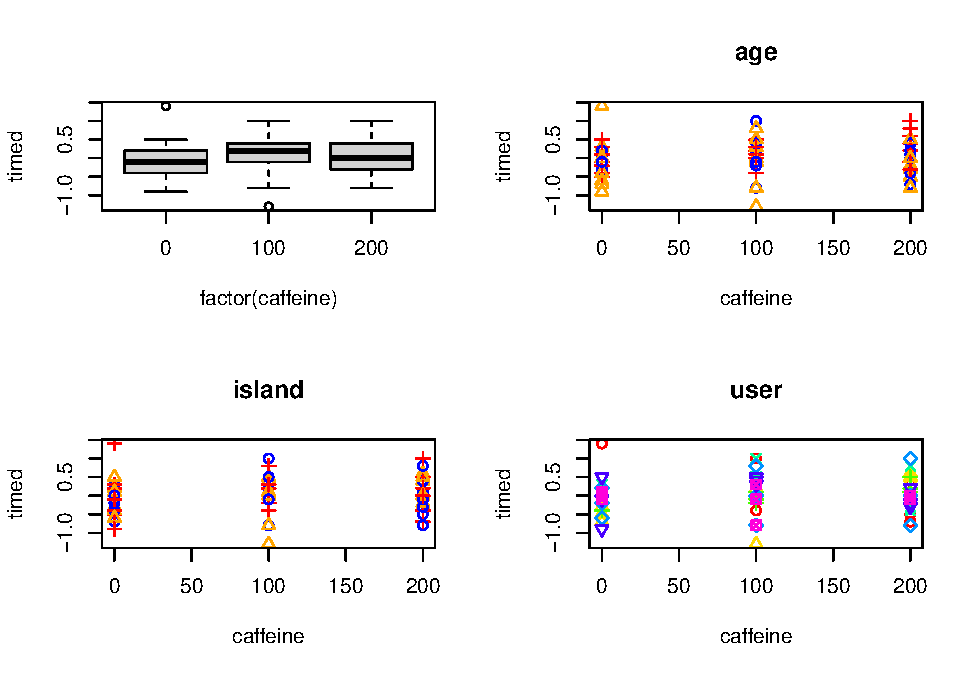
\includegraphics{island_caffeine_files/figure-latex/basic plots-1.pdf}

\begin{Shaded}
\begin{Highlighting}[]
\FunctionTok{par}\NormalTok{(}\AttributeTok{mfrow =} \FunctionTok{c}\NormalTok{(}\DecValTok{1}\NormalTok{, }\DecValTok{2}\NormalTok{))}
\FunctionTok{plot}\NormalTok{(timed }\SpecialCharTok{\textasciitilde{}} \FunctionTok{factor}\NormalTok{(age))}
\FunctionTok{plot}\NormalTok{(timed }\SpecialCharTok{\textasciitilde{}} \FunctionTok{factor}\NormalTok{(island))}
\end{Highlighting}
\end{Shaded}

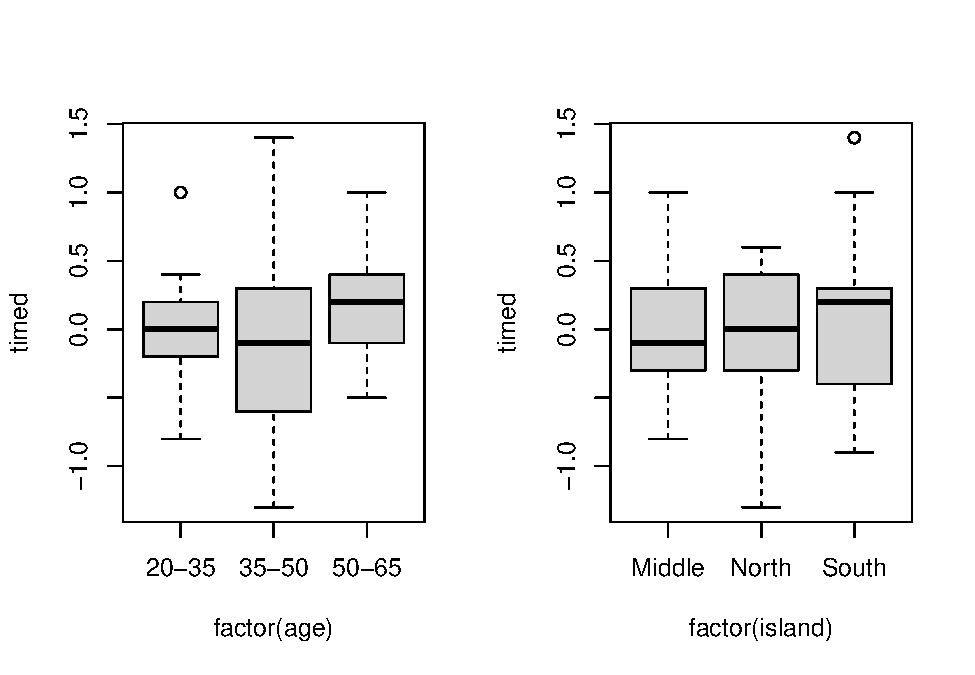
\includegraphics{island_caffeine_files/figure-latex/basic plots-2.pdf}

\begin{Shaded}
\begin{Highlighting}[]
\FunctionTok{par}\NormalTok{(}\AttributeTok{mfrow =} \FunctionTok{c}\NormalTok{(}\DecValTok{1}\NormalTok{, }\DecValTok{1}\NormalTok{))}
\FunctionTok{plot}\NormalTok{(timed }\SpecialCharTok{\textasciitilde{}} \FunctionTok{factor}\NormalTok{(user))}
\end{Highlighting}
\end{Shaded}

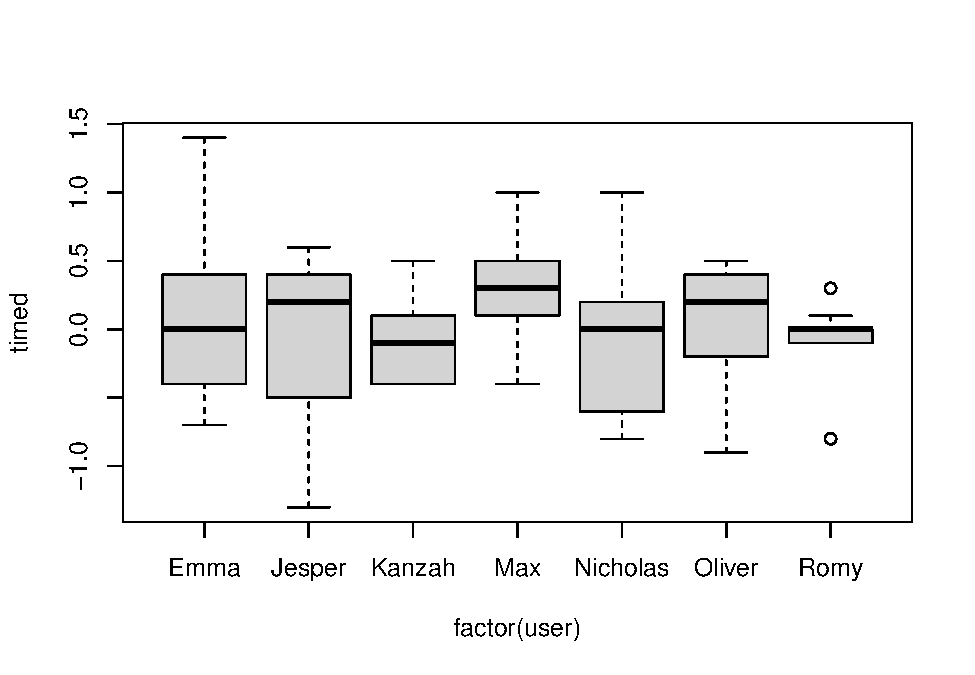
\includegraphics{island_caffeine_files/figure-latex/basic plots-3.pdf}

\subsubsection{d) Sample Size and Power}\label{d-sample-size-and-power}

\begin{Shaded}
\begin{Highlighting}[]
\NormalTok{mean0 }\OtherTok{\textless{}{-}} \FunctionTok{mean}\NormalTok{(timed[caffeine }\SpecialCharTok{==} \DecValTok{0}\NormalTok{])}
\NormalTok{mean1 }\OtherTok{\textless{}{-}} \FunctionTok{mean}\NormalTok{(timed[caffeine }\SpecialCharTok{==} \DecValTok{100}\NormalTok{])}
\NormalTok{mean2 }\OtherTok{\textless{}{-}} \FunctionTok{mean}\NormalTok{(timed[caffeine }\SpecialCharTok{==} \DecValTok{200}\NormalTok{])}

\NormalTok{caffeine\_range }\OtherTok{\textless{}{-}} \FunctionTok{range}\NormalTok{(}\FunctionTok{c}\NormalTok{(mean0, mean1, mean2))}
\NormalTok{caffeine\_range}
\end{Highlighting}
\end{Shaded}

\begin{verbatim}
## [1] -0.07619048  0.09047619
\end{verbatim}

\begin{Shaded}
\begin{Highlighting}[]
\NormalTok{d }\OtherTok{\textless{}{-}} \FunctionTok{abs}\NormalTok{(}\FunctionTok{diff}\NormalTok{(caffeine\_range))}
\NormalTok{mse }\OtherTok{\textless{}{-}} \FunctionTok{summary}\NormalTok{(timed\_aov)[[}\DecValTok{1}\NormalTok{]][[}\StringTok{"Mean Sq"}\NormalTok{]][}\DecValTok{5}\NormalTok{]}
\NormalTok{caf\_sd }\OtherTok{\textless{}{-}} \FunctionTok{sqrt}\NormalTok{(mse)}
\NormalTok{f }\OtherTok{\textless{}{-}}\NormalTok{ d }\SpecialCharTok{/}\NormalTok{ caf\_sd}

\NormalTok{caffeine\_min }\OtherTok{\textless{}{-}} \FunctionTok{pwr.anova.test}\NormalTok{(}\AttributeTok{k =} \DecValTok{3}\NormalTok{, }\AttributeTok{f =}\NormalTok{ f, }\AttributeTok{sig.level =} \FloatTok{0.05}\NormalTok{, }\AttributeTok{power =} \FloatTok{0.8}\NormalTok{)}
\NormalTok{caffeine\_min}
\end{Highlighting}
\end{Shaded}

\begin{verbatim}
## 
##      Balanced one-way analysis of variance power calculation 
## 
##               k = 3
##               n = 33.72766
##               f = 0.3133475
##       sig.level = 0.05
##           power = 0.8
## 
## NOTE: n is number in each group
\end{verbatim}

\begin{Shaded}
\begin{Highlighting}[]
\NormalTok{caffeine\_pwr }\OtherTok{\textless{}{-}} \FunctionTok{pwr.anova.test}\NormalTok{(}\AttributeTok{k =} \DecValTok{3}\NormalTok{, }\AttributeTok{n =} \DecValTok{21}\NormalTok{, }\AttributeTok{f =}\NormalTok{ f, }\AttributeTok{sig.level =} \FloatTok{0.05}\NormalTok{)}
\NormalTok{caffeine\_pwr}
\end{Highlighting}
\end{Shaded}

\begin{verbatim}
## 
##      Balanced one-way analysis of variance power calculation 
## 
##               k = 3
##               n = 21
##               f = 0.3133475
##       sig.level = 0.05
##           power = 0.5751066
## 
## NOTE: n is number in each group
\end{verbatim}

\begin{Shaded}
\begin{Highlighting}[]
\NormalTok{caf\_n }\OtherTok{\textless{}{-}}\NormalTok{ caffeine\_min}\SpecialCharTok{$}\NormalTok{n}
\NormalTok{caf\_pwr }\OtherTok{\textless{}{-}}\NormalTok{ caffeine\_pwr}\SpecialCharTok{$}\NormalTok{power}
\end{Highlighting}
\end{Shaded}

\paragraph{i) Minimum and Maximum
means}\label{i-minimum-and-maximum-means}

The minimum and maximum means of the treatment group are
\(-0.0761905, 0.0904762\).

\paragraph{ii) Standard Deviation}\label{ii-standard-deviation}

A preliminary estimate of \(\sigma^2\) is obtained from \(MS_E\) which
is \(\hat\sigma^2 = 0.2829079\). Therefore, we have that
\(\sigma = 0.5318909\).

\paragraph{iii) Justifying Sample
Size}\label{iii-justifying-sample-size}

From \texttt{pwr.anova.test()}, \(n = 33.72766\), so for 0.8 test power,
\(n=34\) replicates are required which is a sample size of \(N=102\).

\paragraph{vi) Reporting Test Power}\label{vi-reporting-test-power}

Since there are \(k=3\) treatment groups and \(n=21\) observations per
group, we have that the power of the test is \(0.5751066\).

\subsection{3. Results and
interpretation}\label{results-and-interpretation}

\subsubsection{a) Summary}\label{a-summary}

\begin{Shaded}
\begin{Highlighting}[]
\FunctionTok{summary}\NormalTok{(timed\_aov)}
\end{Highlighting}
\end{Shaded}

\begin{verbatim}
##                  Df Sum Sq Mean Sq F value Pr(>F)
## factor(caffeine)  2  0.341  0.1706   0.603  0.551
## factor(age)       2  0.748  0.3740   1.322  0.276
## factor(island)    2  0.177  0.0883   0.312  0.733
## factor(user)      6  1.113  0.1855   0.656  0.685
## Residuals        50 14.145  0.2829
\end{verbatim}

\subsubsection{b) Diagnostic Plots}\label{b-diagnostic-plots}

\begin{Shaded}
\begin{Highlighting}[]
\FunctionTok{par}\NormalTok{(}\AttributeTok{mfrow =} \FunctionTok{c}\NormalTok{(}\DecValTok{1}\NormalTok{, }\DecValTok{2}\NormalTok{))}
\FunctionTok{plot}\NormalTok{(timed\_aov, }\AttributeTok{which =} \FunctionTok{c}\NormalTok{(}\DecValTok{1}\NormalTok{, }\DecValTok{2}\NormalTok{))}
\end{Highlighting}
\end{Shaded}

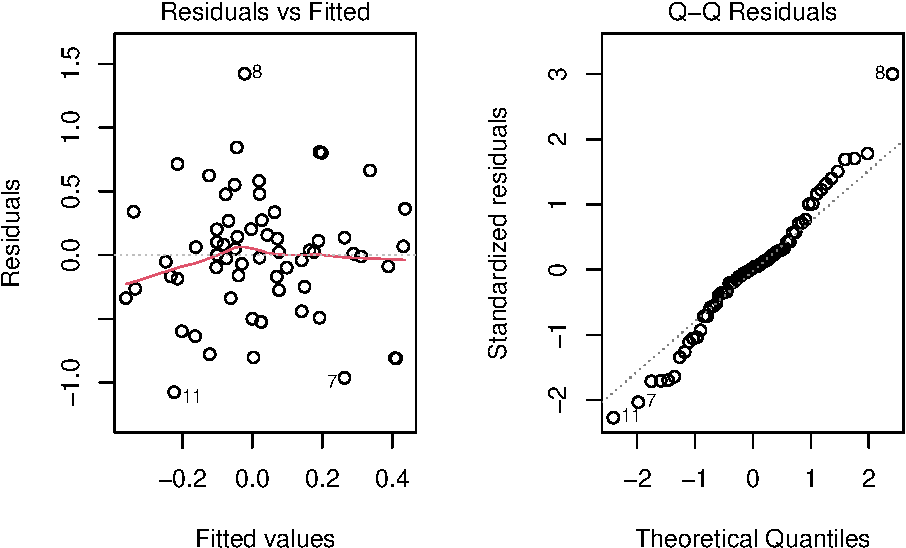
\includegraphics{island_caffeine_files/figure-latex/diagnostic-1.pdf}

\subsubsection{c) Post-hoc Analysis}\label{c-post-hoc-analysis}

\begin{Shaded}
\begin{Highlighting}[]
\FunctionTok{TukeyHSD}\NormalTok{(timed\_aov)}
\end{Highlighting}
\end{Shaded}

\begin{verbatim}
##   Tukey multiple comparisons of means
##     95% family-wise confidence level
## 
## Fit: aov(formula = timed ~ factor(caffeine) + factor(age) + factor(island) + factor(user))
## 
## $`factor(caffeine)`
##                diff        lwr       upr     p adj
## 100-0    0.16666667 -0.2298128 0.5631461 0.5707420
## 200-0    0.14285714 -0.2536223 0.5393366 0.6613427
## 200-100 -0.02380952 -0.4202890 0.3726699 0.9884703
## 
## $`factor(age)`
##                   diff        lwr       upr     p adj
## 35-50-20-35 -0.1428571 -0.5393366 0.2536223 0.6613427
## 50-65-20-35  0.1238095 -0.2726699 0.5202890 0.7324708
## 50-65-35-50  0.2666667 -0.1298128 0.6631461 0.2448666
## 
## $`factor(island)`
##                     diff        lwr       upr     p adj
## North-Middle -0.02857143 -0.4250509 0.3679080 0.9834414
## South-Middle  0.09523810 -0.3012414 0.4917175 0.8312879
## South-North   0.12380952 -0.2726699 0.5202890 0.7324708
## 
## $`factor(user)`
##                        diff        lwr       upr     p adj
## Jesper-Emma     -0.24444444 -1.0145704 0.5256815 0.9571271
## Kanzah-Emma     -0.21111111 -0.9812371 0.5590149 0.9791288
## Max-Emma         0.14444444 -0.6256815 0.9145704 0.9972302
## Nicholas-Emma   -0.18888889 -0.9590149 0.5812371 0.9882205
## Oliver-Emma     -0.10000000 -0.8701260 0.6701260 0.9996557
## Romy-Emma       -0.22222222 -0.9923482 0.5479038 0.9730211
## Kanzah-Jesper    0.03333333 -0.7367927 0.8034593 0.9999995
## Max-Jesper       0.38888889 -0.3812371 1.1590149 0.7130656
## Nicholas-Jesper  0.05555556 -0.7145704 0.8256815 0.9999891
## Oliver-Jesper    0.14444444 -0.6256815 0.9145704 0.9972302
## Romy-Jesper      0.02222222 -0.7479038 0.7923482 1.0000000
## Max-Kanzah       0.35555556 -0.4145704 1.1256815 0.7895800
## Nicholas-Kanzah  0.02222222 -0.7479038 0.7923482 1.0000000
## Oliver-Kanzah    0.11111111 -0.6590149 0.8812371 0.9993690
## Romy-Kanzah     -0.01111111 -0.7812371 0.7590149 1.0000000
## Nicholas-Max    -0.33333333 -1.1034593 0.4367927 0.8348711
## Oliver-Max      -0.24444444 -1.0145704 0.5256815 0.9571271
## Romy-Max        -0.36666667 -1.1367927 0.4034593 0.7650936
## Oliver-Nicholas  0.08888889 -0.6812371 0.8590149 0.9998261
## Romy-Nicholas   -0.03333333 -0.8034593 0.7367927 0.9999995
## Romy-Oliver     -0.12222222 -0.8923482 0.6479038 0.9989142
\end{verbatim}

\end{document}
